\documentclass[preprint,12pt]{elsarticle}

\usepackage[T1]{fontenc}
\usepackage{lmodern}
\usepackage{microtype}
\usepackage{amsmath,amssymb,bm,graphicx}
\graphicspath{{../figures/}}
\usepackage{booktabs}
\usepackage{hyperref}
\usepackage{orcidlink}
\newcommand{\dd}{\mathrm{d}}
\emergencystretch=4em
\renewcommand{\theequation}{S\arabic{equation}}
\renewcommand{\thesection}{S\arabic{section}}
\renewcommand{\thefigure}{S\arabic{figure}}
\renewcommand{\thetable}{S\arabic{table}}

\journal{International Journal of Heat and Mass Transfer}

\begin{document}

\begin{frontmatter}

\title{Supplementary Material for\\ ``Classical heat exchanger fouling-resistance laws as first-moment identities of additive stochastic deposition''}

\author[cog]{Simone Casolo\,\orcidlink{0000-0003-2945-8931}}
\affiliation[cog]{organization={Cognite},
            addressline={John Strandruds vei 10},
            postcode={1360},
            city={Fornebu},
            country={Norway}}

\end{frontmatter}

\section{Notation}
\label{app:notation}

The deposition $D(t)$ is a subordinator with L\'evy measure $\nu(\dd x)$ on
$(0,\infty)$, activity $r=\int\nu(\dd x)$ and cumulant rates
$q_n=\int_0^\infty x^n\,\nu(\dd x)$, so that $\kappa_n[D(t)]=q_nt$. Its law is
fixed by the Laplace exponent through
$\mathbb E[e^{-\theta D(t)}]=e^{-t\Phi(\theta)}$ with
\begin{equation}
  \Phi(\theta)=\int_0^\infty\bigl(1-e^{-\theta x}\bigr)\,\nu(\dd x),
  \qquad\theta\ge0 .
  \label{eq:S_lk}
\end{equation}
We write $m=q_1$ for the mean deposition rate, $s^2=q_2$ for the variance
rate, $c^2=s^2/(m^2\tau_0)$ for the squared coefficient of variation over a
reference window $\tau_0$, $t_c=s^2/m^2$ and $\ell=q_2/q_1=s^2/m=m\,t_c$ for
the size-biased event size. 

\section{Finite activity and the compound Poisson equivalence}
\label{app:cpp_equivalence}

This section proves the equivalence in Sec.~3.1: a
subordinator has finite activity, $r=\int\nu(dx)<\infty$, if and only if it
is a compound Poisson process~\cite{Sato1999,Applebaum2009}. 
It is worth separating the two directions:
finite activity is a statement about the L\'evy measure $\nu$, whereas
being a compound Poisson process is a statement about how the sample path
is assembled from discrete jumps. 

\paragraph*{From finite activity to a Poisson sum of jumps.}
Suppose $r<\infty$. Then $\nu$ splits into an overall rate and a shape,
\begin{equation}
  \nu(dx)=r\,F(dx),
\end{equation}
and $F$ is a probability distribution on $(0,\infty)$, since
$\int F(dx)=r^{-1}\int\nu(dx)=1$. This normalization step is only possible
because $r$ is finite.
 Substituting $\nu=rF$ into the L\'evy--Khintchine exponent, Eq.~\eqref{eq:S_lk}, 
\begin{equation}
  \Phi(\theta)=\int_0^\infty\bigl(1-e^{-\theta x}\bigr)\,r\,F(dx)
  =r\bigl[1-\widehat F(\theta)\bigr].
  \label{eq:cpp_phi}
\end{equation}
All dependence on the jump-size distribution is
now carried by $\widehat F$, where 
$\widehat F(\theta)=\int_0^\infty e^{-\theta x}\,F(dx)$ is the
Laplace transform of $F$.
Insert Eq.~\eqref{eq:cpp_phi} into $\mathbb E[e^{-\theta D(t)}]=e^{-t\Phi(\theta)}$
and expand the exponential in powers of $\widehat F(\theta)$:
\begin{equation}
  \mathbb E\bigl[e^{-\theta D(t)}\bigr]
  =e^{-rt}\,e^{\,rt\widehat F(\theta)}
  =\sum_{n=0}^\infty\underbrace{\frac{(rt)^n e^{-rt}}{n!}}_{\Pr[N(t)=n]}\,
    \widehat F(\theta)^n ,
  \label{eq:cpp_sum}
\end{equation}
where the coefficient of $\widehat F(\theta)^n$ is a
Poisson$(rt)$ probability. This is
exactly the Laplace transform one obtains by conditioning on the
number of jumps: for $N(t)\sim\mathrm{Poisson}(rt)$ and
$X_i\stackrel{\mathrm{iid}}{\sim}F$ independent of $N(t)$,
\begin{equation}
\begin{aligned}
  \mathbb E\Bigl[e^{-\theta\sum_{i=1}^{N(t)}X_i}\Bigr]
  &=\sum_{n=0}^\infty\Pr[N(t)=n]\,
     \mathbb E\Bigl[e^{-\theta\sum_{i=1}^nX_i}\Bigr]\\[2pt]
  &=\sum_{n=0}^\infty\Pr[N(t)=n]\,\widehat F(\theta)^n,
\end{aligned}
\end{equation}
which is term-by-term identical to Eq.~\eqref{eq:cpp_sum}. Since the
Laplace transform determines the law, $D(t)\stackrel{d}{=}\sum_{i=1}^{N(t)}X_i$:
$D$ is, by definition, a compound Poisson process of rate $r$ and jump law
$F=\nu/r$.

\paragraph*{From a Poisson sum of jumps back to finite activity.}
The converse needs no further calculation, only reading the definition in
the other direction. A compound Poisson process of rate $r$ and jump
law $F$ has a L\'evy--Khintchine representation with L\'evy measure
$\nu=r F$; by uniqueness of that representation, this is \emph{the}
L\'evy measure of the process, not merely one that reproduces its law.
Since $F$ is a probability measure, $\int\nu(dx)=r\int F(dx)=r<\infty$:
the process automatically has finite activity, equal to its jump rate.

Put together, the two directions say that the map
$\nu\leftrightarrow(r,F)$ is a bijection between L\'evy measures with
$r<\infty$ and (rate, jump-law) pairs: every finite-activity subordinator
is a compound Poisson process, and every compound Poisson process has
finite activity equal to its own rate. 

\section{Tempered-stable family: derivations}
\label{app:tempered}

This section carries out the five calculations that the tempered-stable
spectrum, Eq.~(13) of the main text, is built to support: fixing the two free scale parameters $B$ and $\lambda$ in terms of the physically meaningful triple $(m,c,\tau_0)$ at any shape $\alpha$; obtaining the
cumulant rates $q_n$, and from them the aggregation scaling of the main text; obtaining the Laplace exponent in
closed form; identifying the three named laws of Table~2 of the main text as three points on this family; and separating three notions---activity, path continuity, and observability---that are easy to conflate. Throughout, $\ell=q_2/q_1$ is the size-biased
event size of the main text: the typical event size as seen by the mass it deposits, rather than by a plain count of events. Only the first calculation, the matching relation Eq.~\eqref{eq:ts_matching}, is needed before any of the others, so a reader interested only in one named law can read that paragraph and then skip ahead.

\paragraph*{Cumulant rates, and matching to $(m,c,\tau_0)$.}
The spectrum $\nu(dx)$ gives the rate at which events of size $x$ occur; its moments $q_n=\int_0^\infty x^n\,\nu(dx)$ are therefore exactly the cumulant rates of the subordinator, with $q_1=m$ the mean deposition rate and $q_2$ the variance rate ($s^2=q_2$ in the notation of the main text). For the tempered-stable spectrum every such moment reduces to a single Gamma-function integral:
\begin{equation}
\begin{aligned}
  q_n&=\int_0^\infty x^n\nu(dx)
      =B\int_0^\infty x^{n-1-\alpha}e^{-\lambda x}\,dx\\[2pt]
     &=B\,\Gamma(n-\alpha)\,\lambda^{\alpha-n},
\end{aligned}
  \label{eq:ts_qn_general}
\end{equation}
valid for every $n\ge1$: the exponential tempering factor $e^{-\lambda x}$ ensures the integral converges at large $x$ regardless of $n$, and the restriction $\alpha<1$ ensures convergence at $x\to0$, which is what keeps even the first moment, $q_1=m$, finite.

Two of these moments are enough to fix both free parameters of the family, $B$ and $\lambda$. Imposing $q_1=m$ sets the overall deposition rate; imposing $q_2/q_1=\ell$ sets the size-biased event size rather than $q_2$ itself, because $\ell$ carries the same units as a jump size and is the more physically transparent quantity to specify. Using $\Gamma(2-\alpha)=(1-\alpha)\Gamma(1-\alpha)$ to simplify the resulting ratio, these two conditions solve to
\begin{equation}
  \lambda=\frac{1-\alpha}{\ell}=\frac{1-\alpha}{c^2m\tau_0},
  \qquad
  B=\frac{m\,\lambda^{1-\alpha}}{\Gamma(1-\alpha)}.
  \label{eq:ts_matching}
\end{equation}
Only two parameters are free in the family, so once $\lambda$ and $B$ are
fixed by $m$ and $\ell$ at a chosen $\alpha$, every higher $q_n$ is
determined by Eq.~\eqref{eq:ts_qn_general}; no further fitting is possible or needed, and $\alpha$ alone governs how the higher cumulants compare to the first two. This dependence can be made explicit without re-evaluating Gamma functions at every $n$. Taking the ratio of
consecutive cumulant rates in Eq.~\eqref{eq:ts_qn_general} gives
$q_n/q_{n-1}=(n-1-\alpha)/\lambda$, and substituting $\lambda=(1-\alpha)/\ell$
from Eq.~\eqref{eq:ts_matching} turns this into a one-step recursion, $q_n/q_{n-1}=(n-1-\alpha)\,\ell/(1-\alpha)$. Iterating the recursion down from $q_1=m$
telescopes it into the closed form
\begin{equation}
  q_n=m\,\ell^{\,n-1}\prod_{k=2}^{n-1}\frac{k-\alpha}{1-\alpha}
  \qquad(n\ge2);
  \label{eq:ts_qn_product}
\end{equation}
the product is empty (equal to $1$) for $n=2$, consistent with $q_2=m\ell$
by the definition of $\ell$ itself---a useful check on the algebra before
using the recursion for $n=3,4$ below.

\paragraph*{Skewness and kurtosis of the increments.}
The third and fourth cumulant rates are the ones most directly tied to data, since they set the skewness and excess kurtosis of the increment distribution over any observation window. Setting $n=3,4$ in
Equation~\eqref{eq:ts_qn_product} gives
\begin{equation}
  \frac{q_3}{q_2}=\frac{2-\alpha}{1-\alpha}\,\ell,
  \qquad
  \frac{q_4}{q_2}=\frac{(2-\alpha)(3-\alpha)}{(1-\alpha)^2}\,\ell^2 .
\end{equation}
These enter the standardized cumulants of a window $\Delta$,
$\gamma_1(\Delta)=q_3q_2^{-3/2}\Delta^{-1/2}$ and
$\gamma_2(\Delta)=q_4q_2^{-2}\Delta^{-1}$, only through the combination
$q_2\Delta=s^2\Delta$, the accumulated variance over the window; this is expected, since $\gamma_1$ and $\gamma_2$ are dimensionless cumulant ratios and $\Delta$ can only enter through how much variance has built up by the end of the window. Writing this out and using $c(\Delta)^2=\ell/(m\Delta)=s^2/(m^2\Delta)$
to trade $\ell$ and $\Delta$ for the single window-dependent coefficient of
variation $c(\Delta)$ reproduces the aggregation scaling of the main text
directly, i.e.\ it is this substitution that the main text's statement of how $\gamma_1$ and $\gamma_2$ shrink with the aggregation window rests on. A useful check that survives this substitution is the ratio
\begin{equation}
  \frac{\gamma_2(\Delta)}{\gamma_1(\Delta)^2}=\frac{q_4q_2}{q_3^{\,2}}=\frac{3-\alpha}{2-\alpha},
\end{equation}
which depends on $\alpha$ alone: $c$ and $\Delta$ cancel because both
$\gamma_1$ and $\gamma_2$ carry the same power of $c(\Delta)$ through
the aggregation scaling of the main text ($\gamma_1\propto c(\Delta)$,
$\gamma_2\propto c(\Delta)^2$), so this ratio is a pure shape diagnostic,
usable in principle to estimate $\alpha$ from data without first knowing $c$,
since it depends only on the shape of the increment distribution and not
on its overall scale.

\paragraph*{Laplace exponent.}
The Laplace exponent
\begin{equation}
  \Phi(\theta)=\int_0^\infty(1-e^{-\theta x})\,\nu(dx),
\end{equation}
already defined in the L\'evy--Khintchine formula, Eq.~\eqref{eq:S_lk}, is the generating function of the subordinator: it determines $\Delta D$'s distribution over any window through $\mathbb{E}[e^{-\theta\Delta D}]=e^{-\Delta\Phi(\theta)}$, and is the object matched below to identify the increment law of each named process. It cannot be obtained by integrating
$x^{-1-\alpha}e^{-\lambda x}$ alone: for $\alpha\ge0$ that integral diverges
at $x=0$, since a single power-law tail with $\alpha\ge0$ carries infinite
activity (infinitely many arbitrarily small events, Sec.~3.1 of the main
text). What converges is the \emph{difference} $1-e^{-\theta x}$ against
the spectrum, because this difference vanishes linearly as $x\to0$ and tames
the singularity that defeats direct integration. Since
$(1-e^{-\theta x})\,e^{-\lambda x}=e^{-\lambda x}-e^{-(\lambda+\theta)x}$, the
tempering already present in $\nu$ turns the integrand into a difference of
two exponentials, each divergent against $x^{-1-\alpha}$ at $x=0$ but with a
convergent difference. This reduces $\Phi$ to the one nontrivial integral
\begin{align}
  \int_0^\infty\bigl(e^{-\lambda x}-e^{-(\lambda+\theta)x}\bigr)\,x^{-1-\alpha}\,dx
  \notag\\
  =\Gamma(-\alpha)\bigl[\lambda^\alpha-(\lambda+\theta)^\alpha\bigr],
  \label{eq:ts_frullani}
\end{align}
a standard tempered-stable identity~\cite{Rosinski2007}, a generalization of
Frullani's integral to a power-law weight. Multiplying
Eq.~\eqref{eq:ts_frullani} by $B$ gives $\Phi(\theta)$ itself, so the only remaining step is to trade $B$ and
$\Gamma(-\alpha)$---both of which are awkward to evaluate directly for
general $\alpha$, the latter diverging at every nonnegative integer---for
the physically meaningful $m$ and $\lambda$ already fixed in
Eq.~\eqref{eq:ts_matching}. Using $\Gamma(1-\alpha)=-\alpha\,\Gamma(-\alpha)$
together with the matching relation $B\,\Gamma(1-\alpha)=m\lambda^{1-\alpha}$
from Eq.~\eqref{eq:ts_matching} eliminates $B$ and $\Gamma(-\alpha)$ in
favor of $m$ and $\lambda$ alone:
\begin{align}
  \Phi(\theta)&=\frac{m\lambda}{\alpha}
    \Bigl[\bigl(1+\theta/\lambda\bigr)^{\alpha}-1\Bigr],
    \qquad\alpha\neq0,
  \label{eq:ts_laplace_exponent}\\
  \Phi(\theta)&=m\lambda\,\ln\bigl(1+\theta/\lambda\bigr),
    \qquad\alpha=0,
  \label{eq:ts_laplace_exponent_gamma}
\end{align}
the $\alpha=0$ case following from the $\alpha\neq0$ one by L'H\^opital's
rule as $\alpha\to0$, since $[(1+\theta/\lambda)^\alpha-1]/\alpha\to\ln(1+\theta/\lambda)$
in that limit.


\begin{figure}[t]
\centering
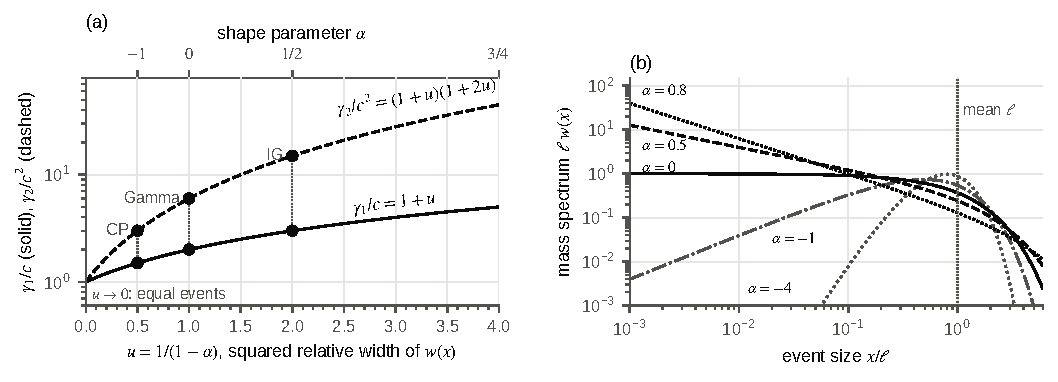
\includegraphics[width=\textwidth]{figS1_alpha_continuum.pdf}
\caption{The tempered-stable family as a continuum, at common $m$, $c$ and
$\tau_0$. (a)~Standardized skewness and excess kurtosis, in units of
$c(\Delta)$ and $c(\Delta)^2$, against $u=1/(1-\alpha)$ (top axis: $\alpha$):
$\gamma_1/c=1+u$, $\gamma_2/c^2=(1+u)(1+2u)$. Compound Poisson, Gamma and
inverse Gaussian ($u=\tfrac12,1,2$; markers) lie on these curves, and
$u\to0$ approaches the bound $\gamma_1\ge c$. (b)~Mass spectrum
$w(x)$ for five values of $\alpha$, all with mean $\ell$ (dotted): $\alpha$
redistributes the deposit between few large and many small events at fixed
mean and variance rate.}
\label{fig:S_alpha}
\end{figure}


\paragraph*{Mass-weighted spectrum.}
The spectrum $\nu(x)$ weights every event by how often it occurs, not by
how much mass it carries, so a large rare event and a small common one can
have the same $\nu(x)$ while contributing very differently to the deposit.
To see the spectrum from the standpoint of mass rather than event count,
multiply the event-rate density by the size $x$ and normalize by the mean
rate $m$: this turns $\nu$ into a genuine probability density,
$w(x)=x\,\nu(x)/m$, giving the fraction of deposited mass that arrives in
events of size near $x$:
\begin{equation}
  w(x)=\frac{\lambda^{1-\alpha}}{\Gamma(1-\alpha)}\,x^{-\alpha}e^{-\lambda x},
\end{equation}
which is recognizable as the $\mathrm{Gamma}(1-\alpha,\lambda)$ density
--- shape $1-\alpha$, rate $\lambda$ --- with mean $(1-\alpha)/\lambda=\ell$
by construction (consistent with $\ell$ being defined as the size-biased,
i.e.\ mass-weighted, event size) and variance $(1-\alpha)/\lambda^2$, i.e.\
relative width (coefficient of variation) $(1-\alpha)^{-1/2}$. This relative
width is governed by $\alpha$ alone, independently of $m$ and $\ell$: the
mass spectrum narrows as $\alpha\to-\infty$, concentrating the deposit into
a few near-identical events, and broadens as $\alpha\to1$, spreading it over
an increasingly wide range of event sizes. This is the precise
sense in which $\alpha$ ``controls how the deposit is distributed over
event sizes'' in Sec.~3.2 of the main text.

\paragraph*{The three named laws.}
The tempered-stable family is a one-parameter continuum in $\alpha$, but
three particular values recover subordinators with well-known, independently
derived increment distributions. Evaluating
Eqs.~\eqref{eq:ts_matching}--\eqref{eq:ts_laplace_exponent_gamma}
at these three values of $\alpha$ recovers the three named processes,
identified by matching $\Phi$ above against their known Laplace exponents
term by term; once $\Phi$ matches, the increment law over any window
$\Delta$ follows immediately, since the Laplace exponent determines the
distribution uniquely. Beyond the algebra, the three laws correspond to
three qualitatively different pictures of how the deposit actually
accumulates, set by how far $\alpha$ has pushed the event-size spectrum
toward few-and-large or many-and-small events (Mass-weighted spectrum,
above); it is worth stating each picture in words before the matching
calculation that confirms it:
\begin{itemize}
  \item $\alpha=-1$ (compound Poisson). Physically, this is the law of a
    surface that sits idle most of the time and then, at random, unrelated
    instants, gains a lump of deposit of random size: nothing happens
    between events, and when something does happen, its size is drawn
    independently of everything else. Concretely, the waiting time between
    successive events is exponential (events occur at a constant rate, with
    no memory of how long it has already been quiet), and each event's size
    is itself exponentially distributed, independently of the waiting
    times and of all other events. It is this combination---a finite,
    constant rate of occurrence together with jumps that occur strictly one
    at a time---that produces the quiescent stretches visible in Fig.~2(d)
    of the main text: genuine flat intervals of the process, not merely
    small increments. Algebraically, substituting $\alpha=-1$ into
    Eq.~\eqref{eq:ts_matching} gives $\lambda=2/\ell$ and
    $B=m\lambda^2$, so by the finite-activity criterion of
    Sec.~3.1 of the main text the total event rate is
    $r=\int\nu(dx)=B/\lambda=2/t_c$: events of all sizes occur at a finite
    combined rate, as required for a list of discrete events to exist at
    all. This lets
    Sec.~\ref{app:cpp_equivalence} apply directly: the normalized
    jump law is $F(dx)=\nu(dx)/r=\lambda e^{-\lambda x}dx$, exponential of
    mean $1/\lambda=\ell/2$, so $\Delta D=\sum_{i=1}^{N}J_i$ with
    $N\sim\mathrm{Poisson}(r\Delta)$ and $J_i\stackrel{\mathrm{iid}}{\sim}\mathrm{Exp}(\mathrm{mean}=\ell/2)$,
    confirming in symbols the picture above: a Poisson-distributed number
    of events, each an independent draw from an exponential jump-size
    distribution. More generally, any
    $\alpha<0$---not only $\alpha=-1$---keeps $r<\infty$ and
    the same idle-then-jump picture, only with the jump size now
    $F$ a $\mathrm{Gamma}(\mathrm{shape}=-\alpha,\mathrm{rate}=\lambda)$-distributed
    draw rather than a plain exponential; writing $a=-\alpha$ for the shape, the aggregation scaling of the main text
    gives $\gamma_1/c=(a+2)/(a+1)$, which recovers $3/2$ at $a=1$
    ($\alpha=-1$) above.
  \item $\alpha=0$ (Gamma process). Physically, this is the opposite
    extreme from compound Poisson: instead of occasional large jumps
    separated by quiescent gaps, the surface receives a continuous rain of
    events so frequent and so small that no individual event can be
    pointed to, and no stretch of time is ever truly flat. The record
    still only ever increases (deposition cannot run backward), but it does
    so through an uninterrupted accumulation of infinitesimal contributions
    rather than through discrete, separately identifiable arrivals.
    Formally, $\lambda=1/\ell$ and $B=m\lambda$;
    the activity is infinite ($0\le\alpha<1$), so there is no finite list of
    discrete events to thin or enumerate---the process deposits through a
    dense set of arbitrarily small jumps rather than a countable sequence of
    them, which is the precise sense of ``continuous rain'' above. Even so, $\Phi(\theta)=m\lambda\ln(1+\theta/\lambda)$,
    Eq.~\eqref{eq:ts_laplace_exponent_gamma}, is exactly the Laplace
    exponent of a Gamma process of shape rate $B$ and scale $1/\lambda$,
    for which $\Delta D\sim\mathrm{Gamma}(\mathrm{shape}=B\Delta,\mathrm{scale}=1/\lambda)$:
    the match is read off by comparing this expression term by term against
    the textbook Laplace exponent of a Gamma process. Since $B\Delta=m\Delta/\ell=\Delta/t_c$ and $1/\lambda=\ell$, this is
    $\Delta D\sim\mathrm{Gamma}(\mathrm{shape}=\Delta/t_c,\ \mathrm{scale}=\ell)$.
  \item $\alpha=1/2$ (inverse Gaussian process). Physically, this law lies
    beyond the Gamma process: it shares its infinite activity,
    so there are no isolated events or quiescent gaps either, but its mass
    spectrum is broader (Mass-weighted spectrum, above), so a somewhat
    larger share of the deposit is carried by comparatively rarer,
    comparatively larger contributions riding on top of the same dense
    background of infinitesimal ones---a bursty, rather than perfectly
    smooth, continuous accumulation. (The inverse Gaussian process also has
    an independent, well-known construction as the first-passage time of a
    drifting Brownian motion through a fixed level, which is a separate
    fact about the law and not how it is derived here.) Formally,
    $\lambda=1/(2\ell)$
    and, from Eq.~\eqref{eq:ts_matching} with $\Gamma(1/2)=\sqrt\pi$,
    $B=m\sqrt{\lambda/\pi}$; by the same term-by-term matching,
    $\Phi(\theta)=2m\lambda[(1+\theta/\lambda)^{1/2}-1]$
    is exactly the Laplace exponent of an inverse Gaussian process, for
    which $\Delta D\sim\mathrm{IG}(\mu_\Delta=m\Delta,\lambda_{\mathrm{IG}}=m\Delta^2/t_c)$.
    As a consistency check, its variance $\mu_\Delta^3/\lambda_{\mathrm{IG}}=c^2m^2\tau_0\Delta$
    agrees with the variance rate of the main text, as it must since both
    were fixed by the same matching condition $q_2/q_1=\ell$.
\end{itemize}
Figure~\ref{fig:S_alpha} places the three
laws on one continuous family, showing both how their skewness and
kurtosis compare (panel a) and how the underlying mass spectrum $w(x)$
reshapes itself as $\alpha$ sweeps between them (panel b). Panel (a) shows
$\gamma_1/c$ approaching, but never crossing, the value $1$ as the mass
spectrum degenerates toward equal-sized events ($u\to0$, i.e.\
$\alpha\to-\infty$, where every event carries the same size). This
floor is not special to the tempered-stable family: it is a general
property of every subordinator, as Sec.~\ref{app:skew_bound} shows.


\paragraph*{Activity, path continuity and observability.}
\label{app:three_distinctions}
The results above are easy to over-interpret, because they blur together
three properties of the family that are logically independent and should
be kept apart.

\emph{Activity} is the event count: finite for $\alpha<0$, where the
process can be written as a genuine list of discrete jumps as in the
compound Poisson case above, and infinite for $\alpha\ge0$, where it
cannot. \emph{Path continuity} is a separate matter and does not track
activity: every member of the family, finite or infinite activity alike, is
a pure-jump process, so the Gamma and inverse-Gaussian paths---despite
having infinite activity---are not continuous but strictly increasing
through a dense set of arbitrarily small jumps. In particular, the Gamma
process is a continuum limit only in this measure-theoretic sense of
infinitely many infinitesimal jumps, and not in the sense of a deposit
thickening smoothly and uniformly the way a continuous function would; no
member of the family has continuous sample paths. \emph{Observability} is a
third, and independent, question again: whether any of the first two
properties can actually be resolved from a measured record depends on the
sampling interval and the measurement noise, and for an area-averaged
thermal resistance it cannot (main text, Sec.~5), regardless of the true
activity or path structure of the underlying process. The quiescent
stretches that distinguish compound Poisson in Fig.~2(d) of the main text
illustrate this: they are a statement about the model's event count
(activity), not a prediction that a measured record will show matching
flat intervals, since the measurement itself may not resolve them.

\subsection{Skewness bound}
\label{app:skew_bound}

For any subordinator, the Cauchy--Schwarz inequality
$q_2^2\le q_1q_3$ gives $\gamma_1(\Delta)\ge c(\Delta)$, with equality only
if all events have the same size (approached as $\alpha\to-\infty$ in the family above):
no matter how the event-size spectrum is shaped, the skewness of the
increments can never fall below the coefficient of variation itself.

\emph{Proof.}
With the window cumulants $\kappa_n=q_n\Delta$,
\begin{equation}
\begin{aligned}
  c(\Delta)&=\frac{\sqrt{q_2\Delta}}{q_1\Delta},\qquad
  \gamma_1(\Delta)=\frac{q_3\Delta}{(q_2\Delta)^{3/2}},\\
  \frac{\gamma_1(\Delta)}{c(\Delta)}&=\frac{q_1q_3}{q_2^{2}},
\end{aligned}
  \label{eq:S_skew_ratio}
\end{equation}
so the ratio is independent of the window and depends on the event-size
spectrum alone. Writing $x^2=x^{1/2}x^{3/2}$ and applying the
Cauchy--Schwarz inequality with respect to $\nu$,
\begin{equation}
\begin{aligned}
  q_2&=\int_0^\infty x^{1/2}x^{3/2}\,\nu(dx)\\
  &\le\Bigl(\int_0^\infty x\,\nu(dx)\Bigr)^{1/2}
     \Bigl(\int_0^\infty x^{3}\,\nu(dx)\Bigr)^{1/2}
  =\sqrt{q_1q_3},
\end{aligned}
\end{equation}
which is $\gamma_1\ge c$. Equality requires $x^{1/2}\propto x^{3/2}$ on the
support of $\nu$, i.e.\ a single event size: compound Poisson with fixed
jumps attains $\gamma_1=c$, and any spread of sizes raises $\gamma_1/c$
above $1$. In the tempered-stable family $\gamma_1/c=1+u$, i.e.\ $1.5$, $2$
and $3$ for the compound Poisson, Gamma and inverse Gaussian laws, and the
bound is approached only as $u\to0$ [Fig.~\ref{fig:S_alpha}(a)].

Physically, a deposit that grows only by adding non-negative pieces must
have increments at least as right-skewed as they are dispersed. A Gaussian
increment model, with zero skewness and finite spread, is therefore never
an exact additive law, only its large-window limit, in which both
$\gamma_1$ and $c$ vanish as $\Delta^{-1/2}$. Conversely, measured
increments whose skewness falls clearly below their coefficient of
variation cannot come from additive deposition alone: measurement noise,
removal or a non-additive mechanism must contribute.

\section{Removal: derivations}
\label{app:removal}

\label{app:linear_removal}
\paragraph*{Cumulants of the L\'evy-driven Ornstein--Uhlenbeck process.}
For a L\'evy process $D$ and a deterministic kernel $f$, the cumulants of a
stochastic integral against $D$ are
\begin{equation}
  \kappa_n\!\biggl[\int_0^tf(u)\,dD(u)\biggr]=q_n\int_0^tf(u)^n\,du.
\end{equation}
With $f(u)=e^{-\psi(t-u)}$ this gives
\begin{equation}
  \kappa_n[R(t)]=q_n\int_0^te^{-n\psi(t-u)}du=q_n\,\frac{1-e^{-n\psi t}}{n\psi},
\end{equation}
Eq.~(18) of the main text; the deterministic initial condition contributes
only to the mean. At stationarity, $\kappa_n=q_n/(n\psi)$.

\paragraph*{Stationary plateau.}
The mean obeys $d\mu/dt=m-\psi\mu$ (Table~1 of the main text), so
$\mu_\infty=R_\infty=m/\psi$. Taking $n=2$ above,
\begin{equation}
  \operatorname{Var}[R]_\infty=\kappa_2=\frac{q_2}{2\psi}=\frac{s^2}{2\psi},
\end{equation}
since $q_2=s^2$. The plateau accordingly contains
\begin{equation}
  N_\infty=\frac{R_\infty}{\ell}=\frac{m/\psi}{s^2/m}=\frac{m^2}{\psi s^2}=\frac1{\psi t_c}
\end{equation}
size-biased events (using $t_c=s^2/m^2=\ell/m$), and
\begin{equation*}
  \mathrm{CV}_\infty^2
  =\frac{\operatorname{Var}[R]_\infty}{R_\infty^2}
  =\frac{s^2/2\psi}{(m/\psi)^2}
  =\frac{\psi s^2}{2m^2}
  =\frac{\psi t_c}{2}
  =\frac1{2N_\infty},
\end{equation*}
the plateau relations of the main text. The shape of the plateau follows the
same route:
\begin{equation}
\begin{aligned}
  \gamma_{1,\infty}&=\frac{\kappa_3}{\kappa_2^{3/2}}
  =\frac{q_3/3\psi}{(q_2/2\psi)^{3/2}}
  =\frac{2\sqrt2}{3}\,\psi^{1/2}q_3q_2^{-3/2}\\
  &=\frac{2\sqrt2}{3}\,\gamma_1(\psi^{-1}),
\end{aligned}
\end{equation}
and $\gamma_{2,\infty}=\kappa_4/\kappa_2^2=\psi\,q_4q_2^{-2}=\gamma_2(\psi^{-1})$.
Using $\gamma_1(\Delta)=[(2-\alpha)/(1-\alpha)]c(\Delta)$,
$\gamma_2(\Delta)=[(2-\alpha)(3-\alpha)/(1-\alpha)^2]c(\Delta)^2$ and
$c(\psi^{-1})=\sqrt2\,\mathrm{CV}_\infty$ for the tempered-stable family gives
\begin{align*}
  \gamma_{1,\infty}&=\frac43\,\frac{2-\alpha}{1-\alpha}\,\mathrm{CV}_\infty,\\
  \gamma_{2,\infty}&=2\,\frac{(2-\alpha)(3-\alpha)}{(1-\alpha)^2}\,\mathrm{CV}_\infty^2,
\end{align*}
the plateau skewness and kurtosis of the main text.


\paragraph*{Per-element detachment.}
Write the deposition as $D(t)=\int_0^t\!\int_0^\infty x\,N_D(du,dx)$, with
$N_D$ a Poisson random measure of intensity $du\,\nu(dx)$, and mark each atom
with an independent lifetime $\tau\sim\mathrm{Exp}(\psi)$. The marked measure
$N(du,dx,d\tau)$ is again Poisson, with intensity
$du\,\nu(dx)\,\psi e^{-\psi\tau}d\tau$, and the deposit present at time $t$ is
$R(t)=\int\!\int\!\int x\,\mathbf 1_{\{t-u<\tau\}}\,N(du,dx,d\tau)$: each
event leaves as a single intact unit at the end of its lifetime. By Campbell's
theorem~\cite{Campbell1909} the cumulants of a Poisson integral are the integrals of the $n$th
power of the integrand against the intensity,
\begin{equation*}
\begin{aligned}
  \kappa_n[R(t)]&=\int_0^t\!du\int_0^\infty\!x^n\nu(dx)\,\Pr(\tau>t-u)\\
  &=q_n\int_0^te^{-\psi(t-u)}du=q_n\,\frac{1-e^{-\psi t}}{\psi},
\end{aligned}
\end{equation*}
which holds for finite and infinite activity alike, since only the moments
$q_n=\int x^n\nu(dx)$, $n\ge1$, enter. At stationarity
$\kappa_n=q_n/\psi$, $n$ times the Ornstein--Uhlenbeck value $q_n/(n\psi)$.
The difference lies in the integrand: under proportional erosion an event of
size $x$ contributes $x\,e^{-\psi(t-u)}$, whose $n$th power integrates to
$1/(n\psi)$, whereas under per-element detachment it contributes $x$ or nothing,
and $\mathbf 1^n=\mathbf 1$ integrates to $1/\psi$. An event made of many
sub-units detaching independently contributes, by the law of large numbers,
its surviving fraction $x\,e^{-\psi(t-u)}$, and so returns the
Ornstein--Uhlenbeck cumulants. The plateau shape follows as before:
\begin{equation}
\begin{aligned}
  \gamma_{1,\infty}&=\frac{q_3/\psi}{(q_2/\psi)^{3/2}}=\psi^{1/2}q_3q_2^{-3/2}=\gamma_1(\psi^{-1}),\\
  \gamma_{2,\infty}&=\psi q_4q_2^{-2}=\gamma_2(\psi^{-1});
\end{aligned}
\end{equation}
with $\mathrm{CV}_\infty^2=\psi q_2/m^2=\psi t_c=c(\psi^{-1})^2$ these are
\begin{equation*}
\begin{aligned}
  \gamma_{1,\infty}&=\frac{2-\alpha}{1-\alpha}\,\mathrm{CV}_\infty,\\
  \gamma_{2,\infty}&=\frac{(2-\alpha)(3-\alpha)}{(1-\alpha)^2}\,\mathrm{CV}_\infty^2.
\end{aligned}
\end{equation*}


\paragraph*{Autocorrelation.}
For continuous, per-element and intermittent removal alike the mean equation closes, and
it holds conditionally on the state at an earlier time:
\begin{equation}
  \mathbb E[R(t+\tau)\,|\,R(t)]=R_\infty+(R(t)-R_\infty)e^{-\psi\tau},\qquad\tau>0.
\end{equation}
Multiplying by $R(t)$ and averaging gives
\begin{equation}
  \operatorname{Cov}[R(t),R(t+\tau)]=\operatorname{Var}[R]\,e^{-\psi\tau}.
\end{equation}

\label{app:sloughing}
\paragraph*{Moments under sloughing.}
Applying the generator of the sloughing equation of the main text to $f(R)=R$ and $f(R)=R^2$,
\begin{align}
  \frac{d\mu_1}{dt}&=m-r_s\eta\,\mu_1,\label{eq:S_slough_m1}\\
  \frac{d\mu_2}{dt}&=2m\mu_1+s^2-r_s\eta(2-\eta)\,\mu_2,\label{eq:S_slough_m2}
\end{align}
where the deposition contributes $2R\,m+s^2$ and an event changes $R^2$ by
$-\eta(2-\eta)R^2$. At stationarity $\mu_1=m/(r_s\eta)=R_\infty$ and
$\mu_2=(2m\mu_1+s^2)/[r_s\eta(2-\eta)]$, so that
\begin{equation}
\begin{aligned}
  \operatorname{Var}&=\mu_2-\mu_1^2
   =\frac{2R_\infty^2}{2-\eta}+\frac{s^2}{(2-\eta)\psi}-R_\infty^2\\[2pt]
  &=\frac{s^2}{(2-\eta)\psi}+\frac{\eta}{2-\eta}R_\infty^2,
\end{aligned}
\end{equation}
with $\psi=r_s\eta$, which is the sloughing variance of the main text.
The transient moments of the three removal mechanisms, and of site
blocking, are compared in Fig.~\ref{fig:S_removal}.

\begin{figure}[t]
\centering
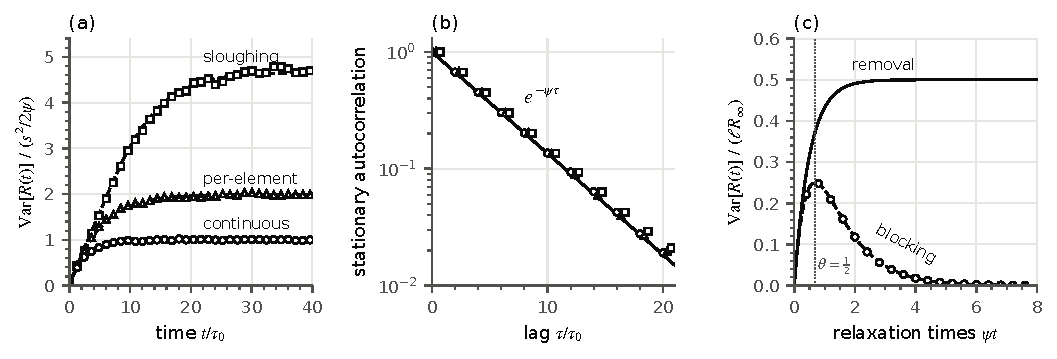
\includegraphics[width=\textwidth]{figS2_removal_moments.pdf}
\caption{Removal mechanisms with the same mean $R_\infty=m/\psi$ and
relaxation rate $\psi$ ($m=c=\tau_0=1$, $\psi=0.2$, Gamma deposition; lines
exact, markers Monte Carlo). (a)~Transient variance, normalized by the
continuous-removal plateau $s^2/2\psi$: continuous removal [Eq.~(18) of the
main text]; per-element detachment, $q_2(1-e^{-\psi t})/\psi$, saturating at
twice that value and half the rate; and sloughing ($\eta=\tfrac12$),
Eqs.~\eqref{eq:S_slough_m1}--\eqref{eq:S_slough_m2}, whose plateau carries a deposition-independent floor.
(b)~All three share
the stationary autocorrelation $e^{-\psi\tau}$, so neither mean nor
correlation time discriminates them. (c)~Independent-site blocking vs.\
continuous removal at the same $R_\infty,\psi$, for equal events of size
$\ell$: removal variance rises monotonically to $\ell R_\infty/2$, while
blocking variance $\ell R_\infty\theta(1-\theta)$ peaks at half coverage and
vanishes at saturation (markers: binomial site filling).}
\label{fig:S_removal}
\end{figure}


\label{app:nonlinear_closure}
\paragraph*{Nonlinear removal.}
Starting from $dR=dD-g(R)\,dt$, the mean and the variance obey
\begin{equation}
  \frac{d\mu}{dt}=m-\mathbb E[g(R)],
  \qquad
  \frac{dV}{dt}=s^2-2\operatorname{Cov}[R,g(R)].
\end{equation}
Expanding $g(R)=g(\mu)+g'(\mu)\delta R+\tfrac12g''(\mu)\delta R^2+\dots$ around
the mean gives, to the order kept by the main text's second-order closure,
\begin{equation}
\begin{aligned}
  \mathbb E[g]&=g(\mu)+\tfrac12g''(\mu)V+O(\kappa_3),\\
  \operatorname{Cov}[R,g(R)]&=g'(\mu)V+O(\kappa_3);
\end{aligned}
\end{equation}
the neglected terms contain the third cumulant and carry the first
dependence on $\alpha$. Explicitly, the next order is
\begin{equation}
\begin{aligned}
  \operatorname{Cov}[R,g(R)]&=g'(\mu)V\\
  &\quad+\tfrac12g''(\mu)\kappa_3[R]+\dots,\\
  \mathbb E[g]&=g(\mu)+\tfrac12g''(\mu)V\\
  &\quad+\tfrac16g'''(\mu)\kappa_3[R]+\dots.
\end{aligned}
\end{equation}
The closure is ordered in $1/N_\infty=\ell/R_\infty$: near the plateau
$V=O(\ell R_\infty)$ and $\kappa_3[R]=O(\ell^2R_\infty)$, i.e.\
$\kappa_n[R]/\mu^n=O(N_\infty^{1-n})$, and with $g^{(j)}\sim g/\mu^{j}$ each
$\kappa_3$ term is smaller than the retained $V$ term of the same equation by
a factor $O(1/N_\infty)$. Dropping $g''\kappa_3$ in the variance equation
while keeping $g''V$ in the mean equation is therefore consistent at leading
order in $1/N_\infty$, although both terms carry $g''$.
Figure~\ref{fig:S_nonlinear} compares the closure with simulation.

\begin{figure}[t]
\centering
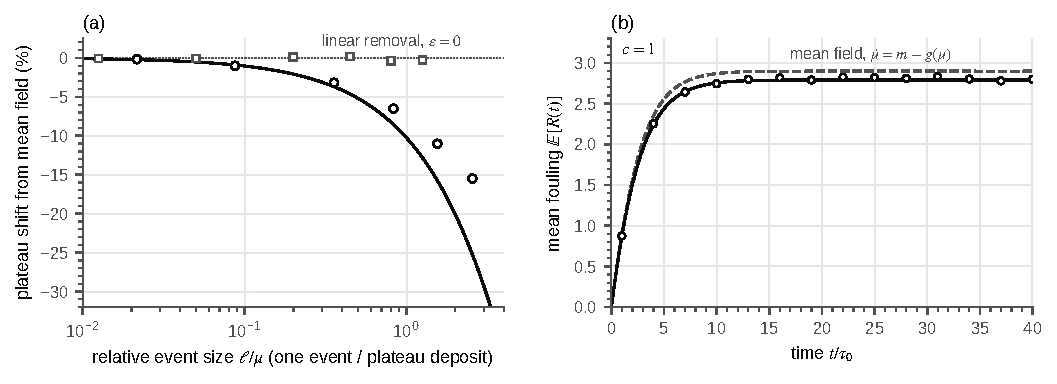
\includegraphics[width=\textwidth]{figS3_nonlinear_removal.pdf}
\caption{Nonlinear removal, $g(R)=\psi R+\varepsilon R^2$ ($m=\tau_0=1$,
$\psi=0.2$, $\varepsilon=0.05$, Gamma deposition). (a)~Shift of the
stationary mean from the mean-field plateau $m=g(\mu)$, against the relative
event size $\ell/\mu$, varied through $c$: second-order closure, Eq.~(26) of
the main text (line), vs.\ Monte Carlo (circles). The closure captures the
shift while the plateau holds many events, and overestimates it once a
single event is comparable to the deposit ($\ell/\mu\gtrsim0.3$), having
dropped $-g''\kappa_3[R]$. Under linear removal ($\varepsilon=0$, squares)
the plateau does not move: only there is the mean universal. (b)~Mean
trajectory at $c=1$: fluctuations lower the plateau from $2.90$ (mean field,
dashed) to $2.81$ (Monte Carlo), against $2.79$ from the closure (solid).}
\label{fig:S_nonlinear}
\end{figure}


\paragraph*{Numerical checks.}
Monte Carlo simulations ($m=c=\tau_0=1$, $\psi=0.2$, $2\times10^4$ paths,
run for $T=60=12\psi^{-1}$ to reach the stationary state) reproduce the stationary skewness of the plateau of the
main text for the three laws ($0.63$, $0.82$,
$1.27$ against $0.63$, $0.84$, $1.27$), the stationary variances of continuous removal, per-element detachment and
sloughing ($2.52$, $5.02$ and $11.61$ against $2.50$, $5.00$ and $11.67$ for
$\eta=0.5$, Gamma deposition, Fig.~\ref{fig:S_removal}; per-element
detachment is simulated exactly by thinning the alive deposit, and the
residuals are within sampling error), the exponential autocorrelation ($0.366$ against
$e^{-1}=0.368$ at $\tau=5$), and the nonlinear plateau of Fig.~\ref{fig:S_nonlinear}.

\section{Granular shot noise and the coefficient of variation}
\label{app:shot_noise}

This section derives the granular estimate of the coefficient of variation
quoted in Sec.~5.2 of the main text, and the area scaling that follows from
it.

\paragraph*{The monodisperse limit of the family.}
In the tempered-stable family, Eq.~(13) of the main text, the mass-weighted spectrum
has relative width $(1-\alpha)^{-1/2}$, so as $\alpha\to-\infty$ it collapses
onto a single size: deposition becomes a compound Poisson process in which
every event deposits the same amount $J_1$. Writing $r$ for the event rate,
the cumulant rates are $q_n=r\,J_1^{\,n}$, so that
\begin{equation}
  m=q_1=r J_1,\qquad s^2=q_2=r J_1^{2},\qquad
  \ell=\frac{q_2}{q_1}=J_1 ,
  \label{eq:S_mono}
\end{equation}
the size-biased event size coinciding with the jump itself, as it must when
all jumps are equal. Substituting $\ell=J_1$ into the squared coefficient of
variation over a window $\Delta$, $c(\Delta)^2=\ell/(m\Delta)$, and evaluating
it at the reference window $\Delta=\tau_0$,
\begin{equation}
  c^{2}=\frac{J_1}{m\,\tau_0}=\frac{1}{r\,\tau_0},
  \label{eq:S_cv_mono}
\end{equation}
one over the mean number of attachments per reference window. This is the
classical shot-noise result for a superposition of Poisson-timed pulses of
equal weight~\cite{Rice1944,Rice1945}; here it is not imported but obtained as
the $\alpha\to-\infty$ member of the family of the main text.

\paragraph*{The size of a single attachment.}
It remains to express $J_1$ for one attached particle. A sphere of diameter
$d_p$ has volume $\pi d_p^{3}/6$. Deposited into a porous layer of solid
fraction $\phi_s$ it occupies a layer volume $(\pi d_p^{3}/6)/\phi_s$;
spread over the heat-transfer area $A$ this raises the deposit thickness by
$\delta_1=(\pi d_p^{3}/6)/(A\phi_s)$, and with $R=\delta/k_f$ the
fouling resistance by
\begin{equation}
  J_1=\frac{\delta_1}{k_f}=\frac{\pi d_p^{3}/6}{A\,\phi_s\,k_f} .
  \label{eq:S_J1}
\end{equation}
Equations~\eqref{eq:S_cv_mono} and \eqref{eq:S_J1} together are the estimate
used in the main text. Nothing in it is adjustable: once $d_p$ and the deposit
properties are fixed, the observed mean rate fixes the event frequency through
$r=m/J_1$.

\paragraph*{Area scaling.}
Because $J_1\propto A^{-1}$ at fixed particle size, Eq.~\eqref{eq:S_cv_mono}
gives $c\propto A^{-1/2}$ at fixed mean rate: granular arrival noise in an
area-averaged observable is suppressed by the square root of the averaging
area. Setting $c=1$ identifies the area on which one sampling period deposits
a single event,
\begin{equation}
  A_1=\frac{\pi d_p^{3}/6}{\phi_s\,k_f\,m\,\tau_0} .
  \label{eq:S_area}
\end{equation}
For $d_p=1~\mu\mathrm{m}$, $k_f=0.5~\mathrm{W\,m^{-1}K^{-1}}$,
$\phi_s=0.5$ and a mean rate of order
$10^{-5}~\mathrm{m^{2}\,K\,W^{-1}}$ per sampling period,
$A_1\approx2\times10^{-13}~\mathrm{m^{2}}$, about a quarter of the
cross-section of the particle itself. That is the sense in which an
area-averaged fouling resistance is deterministic with respect to the
granularity of deposition: order-unity fluctuations would require averaging
over a surface no larger than one grain.

\section{Record length for law identification}
\label{app:record_length}

This section derives the noise attenuation of the standardized cumulants and
the record-length estimate quoted in the main text. Write
\begin{equation}
  \rho=\frac{2\sigma^2}{c^2m^2\tau_0^{2}}
  \label{eq:S_rho}
\end{equation}
for the noise-to-signal ratio. The observed increment over $k$
periods is the sum of the deposition increment, with cumulants
$\kappa_n[\Delta D]=q_nk\tau_0$, and two independent Gaussian measurement
errors of variance $\sigma^2$ each, which contribute only to $\kappa_2$.
Writing $\kappa_2[\Delta y]=\kappa_2[\Delta D](1+\rho/k)$ and substituting
into the standardized cumulants gives
\begin{equation}
  \gamma_{1,k}=\gamma_1\,\frac{k}{(k+\rho)^{3/2}},\qquad
  \gamma_{2,k}=\gamma_2\,\frac{k}{(k+\rho)^{2}}.
  \label{eq:S_atten}
\end{equation}

The windows that best \emph{retain} the cumulants maximize
Eq.~\eqref{eq:S_atten} over $k$. For the skewness,
\begin{equation}
  \frac{d}{dk}\,\frac{k}{(k+\rho)^{3/2}}
  =\frac{(k+\rho)-\tfrac32k}{(k+\rho)^{5/2}}=0
  \quad\Rightarrow\quad k^\ast=2\rho,
\end{equation}
\begin{equation}
\max_k\gamma_{1,k}=\gamma_1\,\frac{2\rho}{(3\rho)^{3/2}}=(2/3\sqrt3)\,\frac{\gamma_1}{\sqrt\rho}.
\end{equation}
For the excess kurtosis,
$(k+\rho)-2k=0$ gives $k^\ast=\rho$ and
$\max_k\gamma_{2,k}=\gamma_2/(4\rho)$. 
Noise-free, the sample estimators numerically
converge on the law-specific values (Fig.~\ref{fig:S_recovery}).

\begin{figure}[t]
\centering
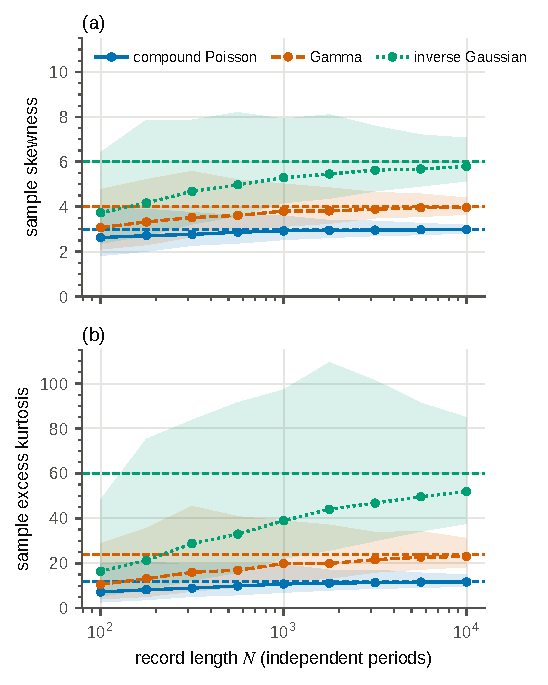
\includegraphics[width=90mm]{figS4_mechanism_recovery.pdf}
\caption{Recovering the microscopic law from skewness and kurtosis:
finite-record convergence of the sample estimators, at $m$, $c=2$, $\tau_0$,
noise-free. For $N$ independent periods (300 Monte Carlo records per $N$),
markers/lines are the median sample skewness (a) and excess kurtosis (b),
shaded bands the $5$--$95\,\%$ range, dashed lines the exact values of
Table~2 of the main text. Both converge onto the correct, law-specific
value within a feasible record length ($N\sim10^2$--$10^3$), given clean
data; for an area-averaged thermal measurement, however, the same
estimators are attenuated by Eq.~\eqref{eq:S_atten}, so the required record
grows to the lengths estimated in Sec.~5.4 of the main text.}
\label{fig:S_recovery}
\end{figure}

Detection requires a second ingredient---the sampling error of the
estimator---and therefore selects a different window. Let two laws differ,
before attenuation, by $\Delta\gamma_1$ or $\Delta\gamma_2$. Each window is
formed from a disjoint pair of observations $k$ periods apart and so consumes
$2k$ periods, giving $n_w=N/(2k)$ independent windows; the standard errors of
the sample skewness and sample excess kurtosis under approximate normality are
$\sqrt{6/n_w}$ and $\sqrt{24/n_w}$. We measure the separation of two
laws in units of the standard error of a \emph{single} estimate: the record is
tested against the value expected under the alternative law, so
$d'=\Delta\gamma_{1,k}/\sqrt{6/n_w}$ and
$d'=\Delta\gamma_{2,k}/\sqrt{24/n_w}$. Comparing two independent records,
the standard error of their difference is larger by $\sqrt2$ and $N$ doubles.
With the attenuated differences
$\Delta\gamma_{1,k}=\Delta\gamma_1\,k/(k+\rho)^{3/2}$ and
$\Delta\gamma_{2,k}=\Delta\gamma_2\,k/(k+\rho)^{2}$ of
Eq.~\eqref{eq:S_atten}, the separability indices are
\begin{equation}
\begin{aligned}
  d'_1&=\Delta\gamma_1\sqrt{\frac{N}{12}}\,\frac{k^{1/2}}{(k+\rho)^{3/2}},\\
  d'_2&=\Delta\gamma_2\sqrt{\frac{N}{48}}\,\frac{k^{1/2}}{(k+\rho)^{2}}.
\end{aligned}
  \label{eq:dprime}
\end{equation}
Setting the derivative of the $k$-dependent factor to zero gives
$\tfrac12(k+\rho)-\tfrac32k=0$, i.e.\ $k=\rho/2$, for the skewness, and
$\tfrac12(k+\rho)-2k=0$, i.e.\ $k=\rho/3$, for the excess kurtosis---both
shorter than $k^\ast$, because a longer window is also a rarer one. At these
windows the factors equal $(2/3\sqrt3)\,\rho^{-1}$ and
$(3\sqrt3/16)\,\rho^{-3/2}$, so that $d'=2$ requires
$N=12\cdot4\cdot(27/4)\,\rho^2/\Delta\gamma_1^2$ and
$N=48\cdot4\cdot(256/27)\,\rho^3/\Delta\gamma_2^2$, that is,
\begin{equation}
  N\gtrsim 324\,\frac{\rho^{2}}{\Delta\gamma_1^{2}},
  \qquad
  N\gtrsim 1820\,\frac{\rho^{3}}{\Delta\gamma_2^{2}}.
  \label{eq:Nreq_general}
\end{equation}
For the Gamma/inverse-Gaussian pair, $\Delta\gamma_1=c$ and
$\Delta\gamma_2=9c^2$ (Sec.~\ref{app:tempered}), giving
$N\approx324\,\rho^2/c^2$ and $N\approx22\,\rho^3/c^4$; the skewness is
therefore the cheaper statistic by a factor $\rho/(14c^{2})$, and it sets the
scaling of the requirement with the noise. Separating windows by one period
instead of $k$ gives $n_w\simeq N/k$ and halves both prefactors without
changing the powers of $\rho$. The estimates are asymptotic in $\rho$:
Fig.~\ref{fig:S_record} tests them by simulation and finds them accurate to
within a factor $1$--$2$ for $\rho\gtrsim10^{2}$ and optimistic below. They
are also specific to moment-based estimation, whereas the attenuation,
Eq.~\eqref{eq:S_atten}, is a property of the measurement and applies to any
estimator.
\begin{figure}[t]
\centering
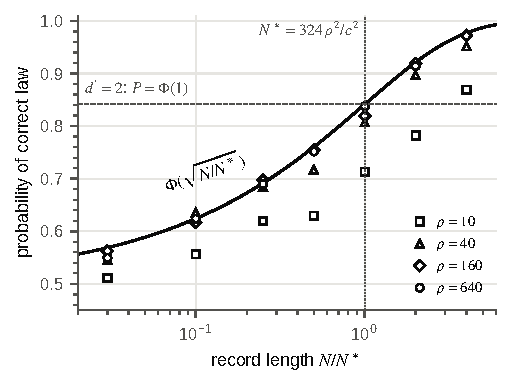
\includegraphics[width=90mm]{figS5_record_validation.pdf}
\caption{Monte Carlo test of the record-length estimate,
Eq.~\eqref{eq:Nreq_general}, for the Gamma and inverse-Gaussian laws at $c=2$.
Each record of $N$ base periods is observed with Gaussian noise set by
$\rho$, Eq.~\eqref{eq:S_rho}, and differenced over $N/2k$ windows of
$k=\rho/2$ periods; the law is assigned by comparing sample skewness with the
midpoint of the two attenuated values, Eq.~\eqref{eq:S_atten}. Markers:
fraction of correct assignments in $1000$ records per law. Line: asymptotic
prediction $\Phi_{\mathrm G}(\sqrt{N/N^\ast})$, with $\Phi_{\mathrm G}$ the standard normal distribution function, i.e.\ $d'=2$ at $N=N^\ast=324\rho^2/c^2$,
which holds for $\rho\gtrsim10^2$ and is optimistic below (about $1.3\times$
longer needed at $\rho=40$, about $3\times$ at $\rho=10$, where $\rho$ is no
longer large compared with $c^2=4$).}
\label{fig:S_record}
\end{figure}
\section{First-passage time: exact distribution and asymptotics}
\label{app:fpt}

\paragraph*{Exact distribution.} Because $R(t)=R_0+D(t)$ is nondecreasing,
$\{T_x\le t\}=\{D(t)\ge x-R_0\}$, and $\Pr(T_x\le t)$ follows directly from the
law of $D(t)$ given in the main text. For the Gamma law,
$D(t)\sim\mathrm{Gamma}(t/(c^2\tau_0),\,c^2m\tau_0)$ and
$\Pr(T_x\le t)=Q\bigl(t/(c^2\tau_0),\,(x-R_0)/(c^2m\tau_0)\bigr)$, the
regularized upper incomplete gamma function. For the compound Poisson law,
conditioning on the number of events $N(t)=n$ gives a sum of $n$
exponential jumps, i.e.\ an Erlang$(n,\ell/2)$ variable, so
$\Pr(D(t)\ge x-R_0\mid N(t)=n)=Q(n,2(x-R_0)/\ell)$; weighting by the
Poisson probabilities of $N(t)$ and summing over $n\ge1$ gives
$\Pr(T_x\le t)$ in closed form. For the inverse Gaussian law,
$D(t)\sim\mathrm{IG}(\mu_t,\lambda_t)$ with $\mu_t=mt$,
$\lambda_t=mt^2/(c^2\tau_0)$, and the standard inverse-Gaussian distribution
function gives $\Pr(T_x\le t)=1-F_{\mathrm{IG}}(x-R_0;\mu_t,\lambda_t)$. All
three reduce, for $x-R_0$ large compared with the event scale $\ell$, to the
normal approximation $\Phi_{\mathrm G}\bigl[(mt-(x-R_0))/(cm\sqrt{\tau_0t})\bigr]$.

\begin{figure}[t]
\centering
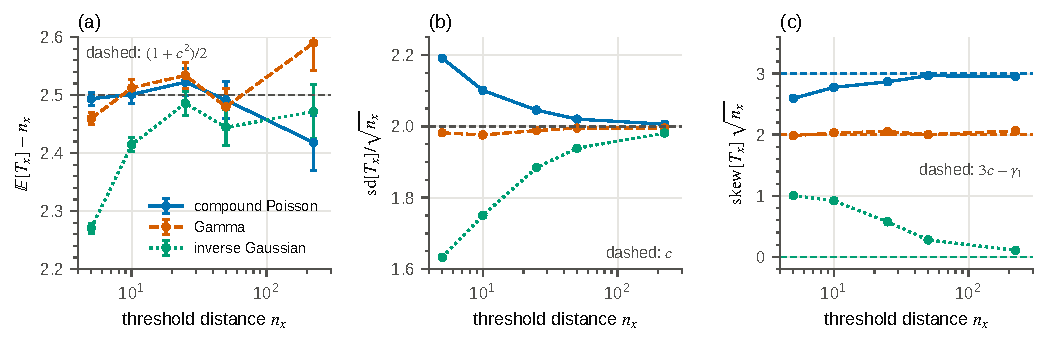
\includegraphics[width=\textwidth]{figS6_fpt_validation}
\caption{Range of validity of the first-passage formulas, by Monte Carlo at
$c=2$ for the three matched laws. (a) $\mathbb E[T_x]-n_x$ vs.\ the predicted
$(1+c^2)/2$ (dashed; error bars $\pm1$ Monte Carlo s.e.). (b)
$\operatorname{sd}[T_x]/\sqrt{n_x}$ vs.\ predicted $c$. (c)
$\operatorname{skew}[T_x]\sqrt{n_x}$ vs.\ predicted $3c-\gamma_1$ (dashed;
zero for the inverse Gaussian law). Accurate at $n_x=220$, degrading towards
small $n_x$, the only regime where the deposition law would matter.}
\label{fig:S_fpt_validation}
\end{figure}

\paragraph*{Asymptotic cumulants.} Write the deposition as a sum of
one-period increments $X_1,X_2,\dots$ with cumulant generating function
$K(\theta)=\log\mathbb E\,e^{\theta X_1}$, mean $\kappa_1=m\tau_0$, variance
$\kappa_2=c^2m^2\tau_0^2$ and third cumulant
$\kappa_3=\gamma_1c^3m^3\tau_0^3$, and let $T=T_x$ be the number of periods
at which the partial sum $S_T=\sum_{i\le T}X_i$ first reaches
$x-R_0$, with overshoot $O=S_T-(x-R_0)\ge0$. For $\theta$ in a neighbourhood
of $0$ where $K$ is finite, $M_n=\exp[\theta S_n-nK(\theta)]$ is a
martingale: since the increments are independent,
$\mathbb E[M_{n+1}\mid X_1,\dots,X_n]=M_n\,\mathbb E[e^{\theta X_{n+1}}]\,e^{-K(\theta)}=M_n$,
and $\mathbb E M_n=M_0=1$. The passage time $T$ is finite with exponential
moments for a subordinator of positive mean, so optional stopping applies and
$\mathbb E M_T=1$; with $S_T=(x-R_0)+O$ this reads
\begin{equation}
  \mathbb E\bigl[e^{\theta(x-R_0)+\theta O-TK(\theta)}\bigr]=1 .
\end{equation}
Choosing $\theta=\theta(u)$ to solve $K(\theta)=-u$ turns $-TK(\theta)$ into
$uT$, and moving the constant factor $e^{\theta(x-R_0)}$ to the right-hand
side gives Wald's identity
\begin{equation}
  \mathbb E\bigl[e^{uT+\theta(u)O}\bigr]=e^{-\theta(u)(x-R_0)}.
  \label{eq:wald_fpt}
\end{equation}
For a distant threshold the overshoot becomes asymptotically independent of
$T$ and converges to the stationary overshoot of renewal theory, with mean
$\mathbb E[O_\infty]=\mathbb E[X_1^2]/(2\kappa_1)=(\kappa_2+\kappa_1^2)/(2\kappa_1)$.
The expectation in Eq.~\eqref{eq:wald_fpt} then factorizes, and its logarithm
is $\log\mathbb E\,e^{uT}=-\theta(u)(x-R_0)-\log\mathbb E\,e^{\theta(u)O_\infty}$.
Since $\theta(u)=-u/\kappa_1+O(u^2)$, the last term is
$-\theta(u)\,\mathbb E[O_\infty]+O(u^2)=u\,\mathbb E[O_\infty]/\kappa_1+O(u^2)$,
so that
\begin{equation}
  \log\mathbb E\,e^{uT}
  =-\theta(u)\,(x-R_0)+\frac{u\,\mathbb E[O_\infty]}{\kappa_1}+O(u^2).
  \label{eq:cgf_fpt}
\end{equation}
Inverting $K(\theta)=-u$ order by order in $u$ (matching
$K(\theta)=\kappa_1\theta+\tfrac12\kappa_2\theta^2+\tfrac16\kappa_3\theta^3+\dots=-u$)
and reading off the coefficients of $u^n/n!$ in
$-\theta(u)(x-R_0)$ gives the cumulants of $T$ to leading order in
$x-R_0$:
\begin{equation}
\begin{aligned}
  \kappa_1(T)&=\frac{x-R_0}{\kappa_1}+O(1),\\[2pt]
  \kappa_2(T)&=\frac{(x-R_0)\,\kappa_2}{\kappa_1^3}+O(1),\\[2pt]
  \kappa_3(T)&=(x-R_0)\Bigl(\frac{3\kappa_2^2}{\kappa_1^5}
              -\frac{\kappa_3}{\kappa_1^4}\Bigr)+O(1).
\end{aligned}
\label{eq:fpt_cumulants}
\end{equation}
Substituting $\kappa_1=m\tau_0$, $\kappa_2=c^2m^2\tau_0^2$,
$\kappa_3=\gamma_1c^3m^3\tau_0^3$ and $n_x=(x-R_0)/(m\tau_0)$ reproduces the
expressions quoted in the main text for the mean and the coefficient of
variation of $T_x$ (in units of $\tau_0$),
and gives for the skewness
\begin{equation}
  \operatorname{skew}[T_x]=\frac{3c-\gamma_1}{\sqrt{n_x}},
  \label{eq:fpt_skewness}
\end{equation}
which is positive whenever $\gamma_1<3c$ (true for the compound Poisson and
Gamma laws at matched $(m,c)$, Sec.~\ref{app:tempered}) and vanishes for
the inverse Gaussian law, whose skewness is exactly $3c$. The $O(1)$
remainders in Eq.~\eqref{eq:fpt_cumulants} come from the overshoot and do
not grow with the distance to the threshold, which is why the leading-order
formulas improve as $n_x$ increases and are least reliable for $n_x$ of
order $10$ or smaller, the regime flagged in the main text.

\paragraph*{Range of validity.} Monte Carlo over $n_x\in\{5,10,25,50,220\}$
(Fig.~\ref{fig:S_fpt_validation}) recovers the mean to within $0.09$ sampling
periods for $n_x\ge10$, but at $n_x=5$ the inverse Gaussian law is biased by
$-0.23$ periods, its spread is $18\,\%$ below $c\sqrt{n_x}$, and its
predicted zero skewness is still $0.45$. At $n_x=220$ the three laws agree
on the mean life to $0.2$ periods and on the $5$th--$95$th percentiles to
$0.9\,\%$. For a threshold within a handful of
increments the life distribution should be simulated rather than taken from
Eqs.~\eqref{eq:fpt_cumulants}--\eqref{eq:fpt_skewness}.



%------------------------------------------------------------------
%\clearpage
\bibliographystyle{elsarticle-num}
\bibliography{references}

\end{document}
